\documentclass[UTF8,11pt,a4paper]{ctexart}
\usepackage[margin=2.15cm,headheight=15pt]{geometry}
\usepackage{amsmath,amssymb,bm}
\usepackage{booktabs,tabularx,array}
\usepackage{graphicx,float,caption,subcaption}
\usepackage{xcolor}
\usepackage{tikz}
\usetikzlibrary{arrows.meta,positioning,fit,calc,shapes.geometric}
\usepackage{hyperref}

\definecolor{navy}{HTML}{17365D}
\definecolor{blue}{HTML}{2F75B5}
\definecolor{cyan}{HTML}{5B9BD5}
\definecolor{orange}{HTML}{ED7D31}
\definecolor{green}{HTML}{70AD47}
\definecolor{lightblue}{HTML}{EAF2F8}
\definecolor{lightgray}{HTML}{F3F5F7}
\definecolor{darkgray}{HTML}{4A4A4A}

\hypersetup{colorlinks=true,linkcolor=navy,urlcolor=blue,citecolor=navy,pdfauthor={HFT Research Project},pdftitle={广义全耦合图模型与GNN复杂参数辨识}}
\pagestyle{plain}
\setlength{\parindent}{2em}
\setlength{\parskip}{0.25em}
\captionsetup{font=small,labelfont=bf}
\graphicspath{{assets/}}
\newcommand{\Yp}{\bm Y_{\mathrm p}}
\newcommand{\Yi}{\bm Y_{\mathrm i}}
\newcommand{\Cps}{C_{\mathrm{ps}}}
\newcommand{\Ls}{L_{\sigma}}
\newcommand{\RR}{\bm R}
\newcommand{\LL}{\bm L}
\newcommand{\CC}{\bm C}
\newcommand{\GG}{\bm G}
\newcommand{\Inc}{\bm A}
\newcommand{\vv}{\bm v}
\newcommand{\ii}{\bm i}

\newenvironment{keybox}{\begin{center}\begin{minipage}{0.91\textwidth}\color{navy}\hrule\vspace{0.55em}\color{black}}{\vspace{0.55em}\color{navy}\hrule\color{black}\end{minipage}\end{center}}

\begin{document}

\begin{titlepage}
\centering
\vspace*{2.2cm}
{\color{navy}\rule{\textwidth}{1.2pt}}\\[1.1cm]
{\fontsize{26}{34}\selectfont\bfseries 广义全耦合图模型与 GNN\\复杂参数辨识}\par
\vspace{0.65cm}
{\Large 从整体互电容到分布式梯形/星形网络的研究收敛}\par
\vspace{1cm}
{\color{navy}\rule{0.72\textwidth}{0.8pt}}\\[1cm]
{\large 阶段实验汇总、矩阵推导、开源工程认知与下一步方案}\par
\vfill
\begin{tabular}{rl}
研究对象：& DAB 工况下高频变压器宽频参数与内部状态\\
核心方法：& 全耦合图表示、可微矩阵求解、Fisher/OED、GNN 结构先验\\
覆盖实验：& 整体 $\Cps$、分布参数、分段、Simscape、四端口、DAB、图物理\\
报告日期：& 2026 年 9 月 6 日
\end{tabular}
\vfill
{\small 本报告基于当前 Git 仓库中 EXP-010 至 EXP-015 及早期可辨识性实验的可复现实验结果整理。}
\end{titlepage}

\tableofcontents
\clearpage

\section{结论先行：GNN 方向应当如何收敛}

当前工作已经不再适合定义成“用一个网络估计总互电容 $\Cps$”。整体 $\Cps$ 的两端口物理反演已经证明可行，真正有研究壁垒的问题是：当经典梯形网络演变为包含非局部互感、非局部跨绕组电容、对地支路和四个独立端子的广义全耦合网络后，如何从有限的端口频响与运行窗口中辨识\textbf{结构化分布参数变化}，同时保持无源性、互易性与内部状态可解释性。

本报告把“星形”限定为一种工程简称：它不是标准的单中心星形电路，而是指梯形局部连接扩展后形成的\textbf{多中心、非局部、全耦合图网络}。经典梯形只是这个图模型的一个稀疏特例。

\begin{keybox}
\textbf{收敛后的核心命题：}建立一个由异构图描述、由矩阵方程精确求解、由 Fisher 信息约束观测分辨率、由 GNN 学习结构先验的逆问题框架。GNN 不替代电路方程，也不能从缺失观测中创造信息；它负责在高维、强相关、变规模的参数空间中学习“哪些边可能变化、哪些变化应共同出现、怎样把端口证据分配到局部边”。
\end{keybox}

因此建议将博士主线写成：
\begin{equation}
\boxed{
\begin{aligned}
&\text{全耦合 HFT 图模型}\rightarrow\text{可微矩阵正演}\rightarrow
\text{Fisher/OED 可辨识分辨率}\\
&\hspace{2.2cm}\rightarrow\text{物理约束 GNN 反演}
\rightarrow\text{端口与内部状态双重验证}
\end{aligned}}
\end{equation}

\section{已有工作形成了怎样的证据链}

\subsection{整体互电容：先证明在线反演与工程量闭环可行}

早期实验基于 Liu 等人的三电容模型，通过固定噪声二值激励恢复传递零点，再反演整体绕组间互电容。基准 $\Cps=28.36\,\mathrm{pF}$，依次并联 $0,2.5,5,10,20\,\mathrm{pF}$；采样率为 $50\,\mathrm{MHz}$，FFT 长度 262144，16 次谱平均，每状态 8 个重复窗口。结果显示平均绝对 $\Cps$ 误差为 $0.746\%$，最小可稳定区分的相邻增量为 $2.5\,\mathrm{pF}$。

\begin{figure}[H]
\centering
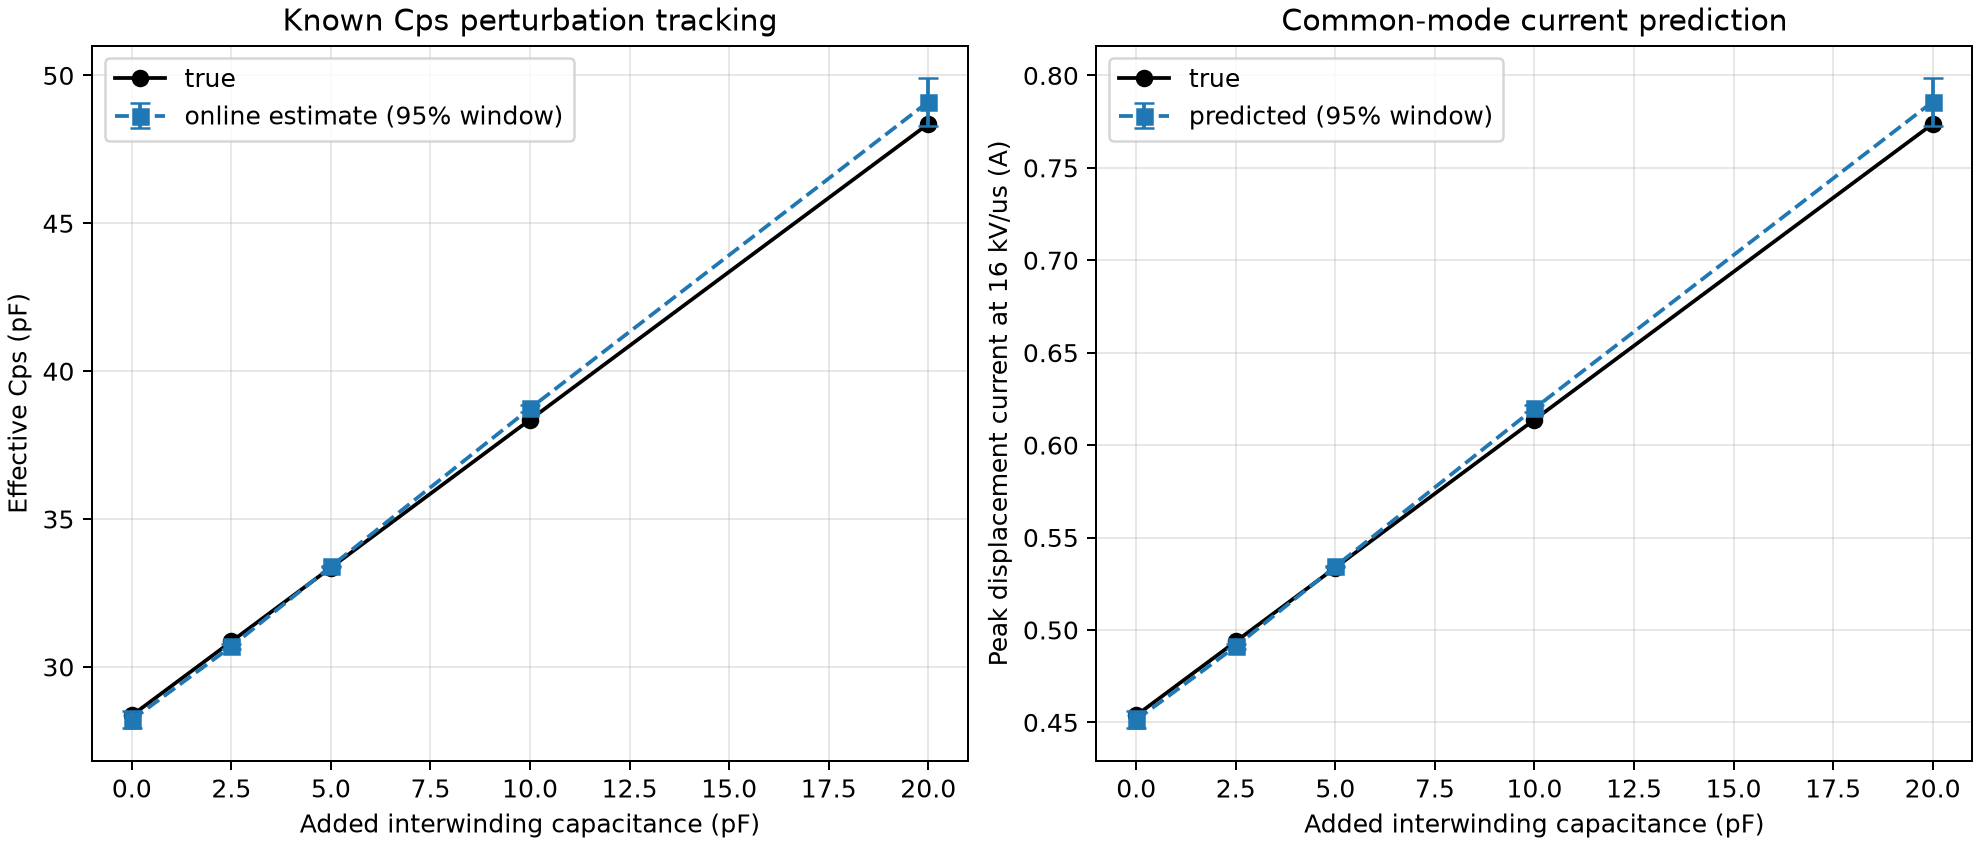
\includegraphics[width=0.94\textwidth]{overall_cps_closure.png}
\caption{整体 $\Cps$ 扰动跟踪与跨绕组位移电流工程闭环。固定 $\mathrm d v/\mathrm dt=16\,\mathrm{kV}/\mu\mathrm{s}$ 时，电流相对误差与电容相对误差相同，这是线性映射的结果，而不是独立的第二个辨识证据。}
\label{fig:overall-cps}
\end{figure}

这一步解决了“\textbf{总量能不能在线估}”的问题，但不能回答“\textbf{互电容分布在哪里发生了变化}”。它应保留为全局辨识基线和 GNN 输出的总量守恒约束：
\begin{equation}
\sum_{(i,j)\in\mathcal E_{ps}} \widehat C_{ps,ij}\approx \widehat C_{ps}^{\mathrm{global}}.
\end{equation}

\subsection{有载 DAB 多端口：证明观测方式比求解器名字更重要}

有载条件下，单端口表观导纳混入副边激励：
\begin{equation}
\frac{I_1}{V_1}=Y_{11}+Y_{12}\frac{V_2}{V_1}.
\end{equation}
因此必须利用多个运行窗口构造端口激励矩阵，并恢复完整两端口导纳：
\begin{equation}
\bm I_k=\bm Y_k\bm V_k,\qquad
\widehat{\bm Y}_k=\bm I_k\bm V_k^H
\left(\bm V_k\bm V_k^H+\lambda\bm I\right)^{-1}.
\end{equation}

已有同模生成--同模反演实验中，联合估计 $\Ls+\Cps$ 的平均误差约为 $0.047\%$；错误单端口方法约为 $85.561\%$，固定错误漏感时平均误差约为 $61.4\%$，$\Ls$ 增加 $5\%$ 时伪 $\Cps$ 误差可达 $159.899\%$。这些数字应理解为\textbf{数值可辨识性基线和错误模型反例}，不能外推为实物精度。

\begin{figure}[H]
\centering
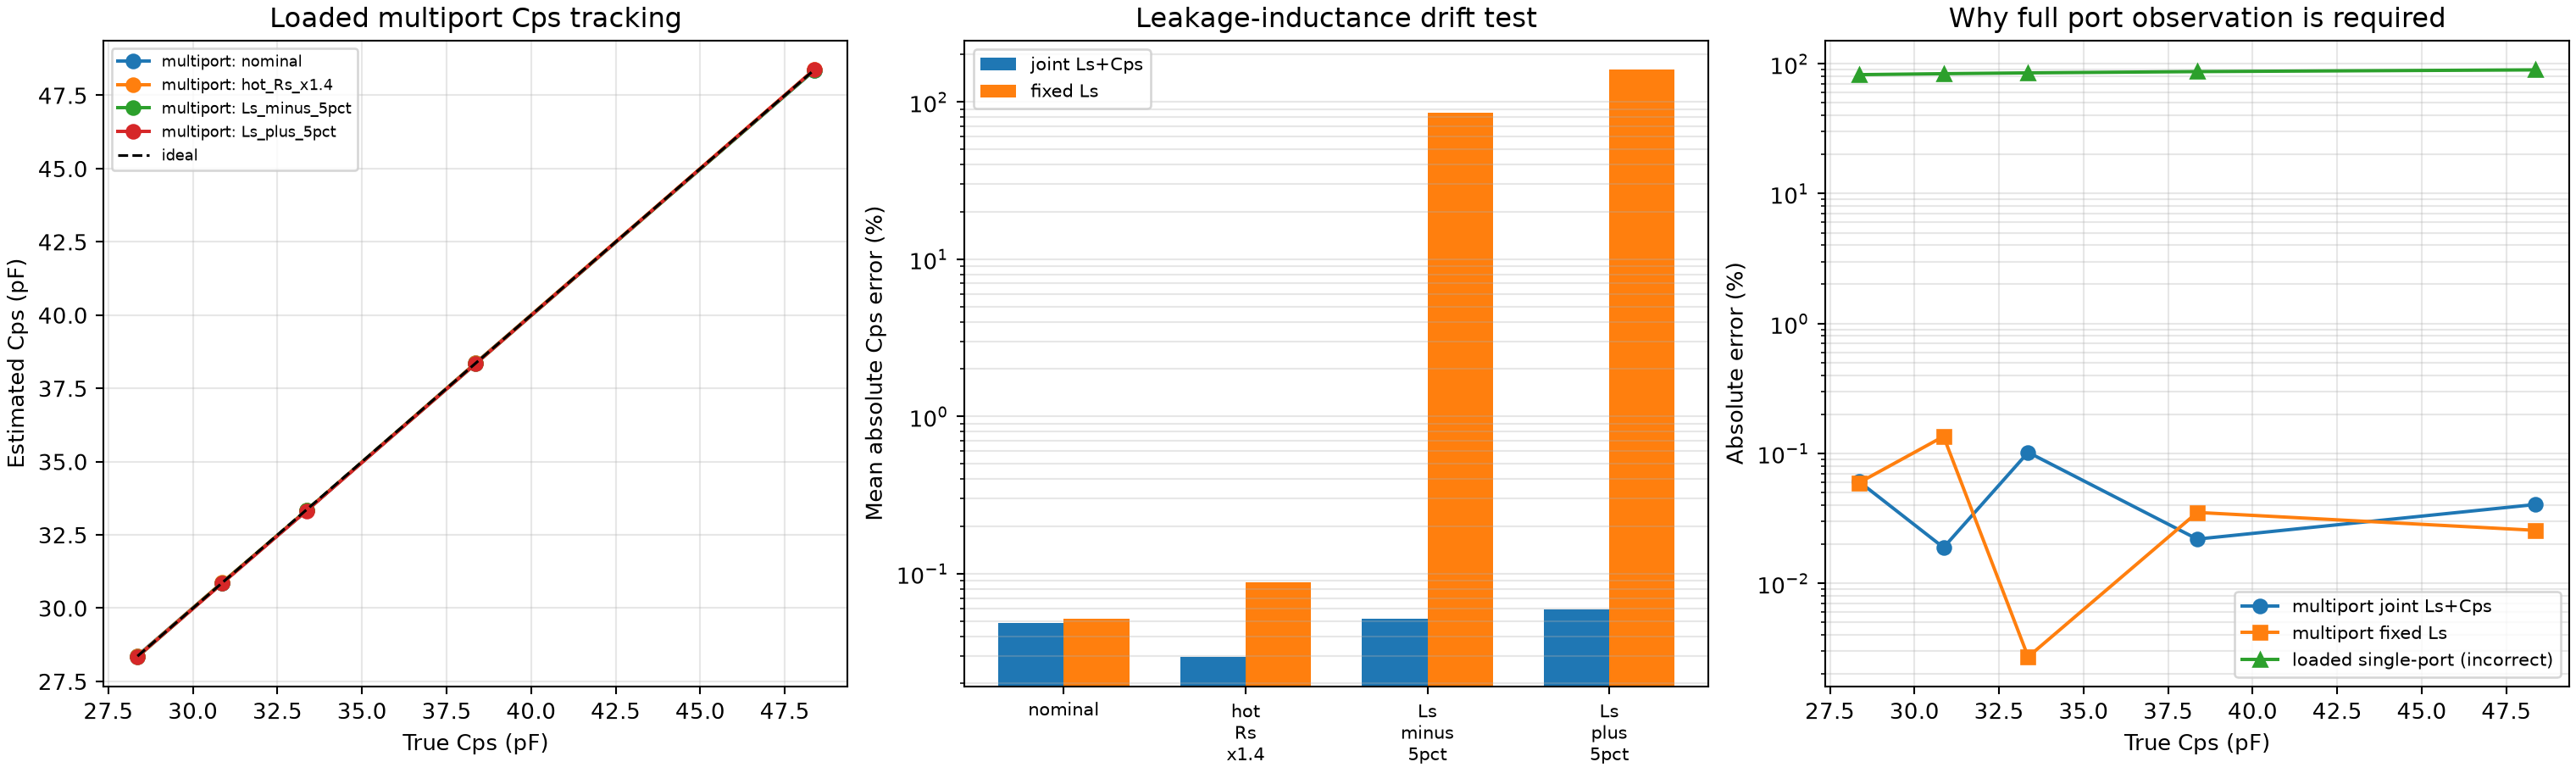
\includegraphics[width=0.96\textwidth]{loaded_multiport_cps.png}
\caption{有载多运行窗口的整体 $\Cps$ 跟踪、漏感漂移反例及完整端口观测必要性。}
\label{fig:loaded-cps}
\end{figure}

\subsection{Fisher/OED：确定信息是否存在，而不是给 GNN 做装饰}

设复数观测向量为 $\bm h_k(\bm\theta)$，对数参数灵敏度为
\begin{equation}
\bm S_k=\frac{\partial\bm h_k}{\partial\log\bm\theta},
\end{equation}
则实参数 Fisher 信息矩阵可写为
\begin{equation}
\bm F=2\operatorname{Re}\sum_{k\in\mathcal K}
\bm S_k^H\bm\Sigma_k^{-1}\bm S_k.
\end{equation}
已有实验表明，仅观测 $Y_{11}$ 或较少自导纳组合时 Fisher 秩不足；加入互导纳 $Y_{12}$ 与另一侧自导纳后，五参数示例可以达到满秩。E-optimal 选频则通过最大化 $\lambda_{\min}(\bm F)$ 避免最弱参数方向被忽略。

\begin{figure}[H]
\centering
\begin{subfigure}[t]{0.47\textwidth}
\centering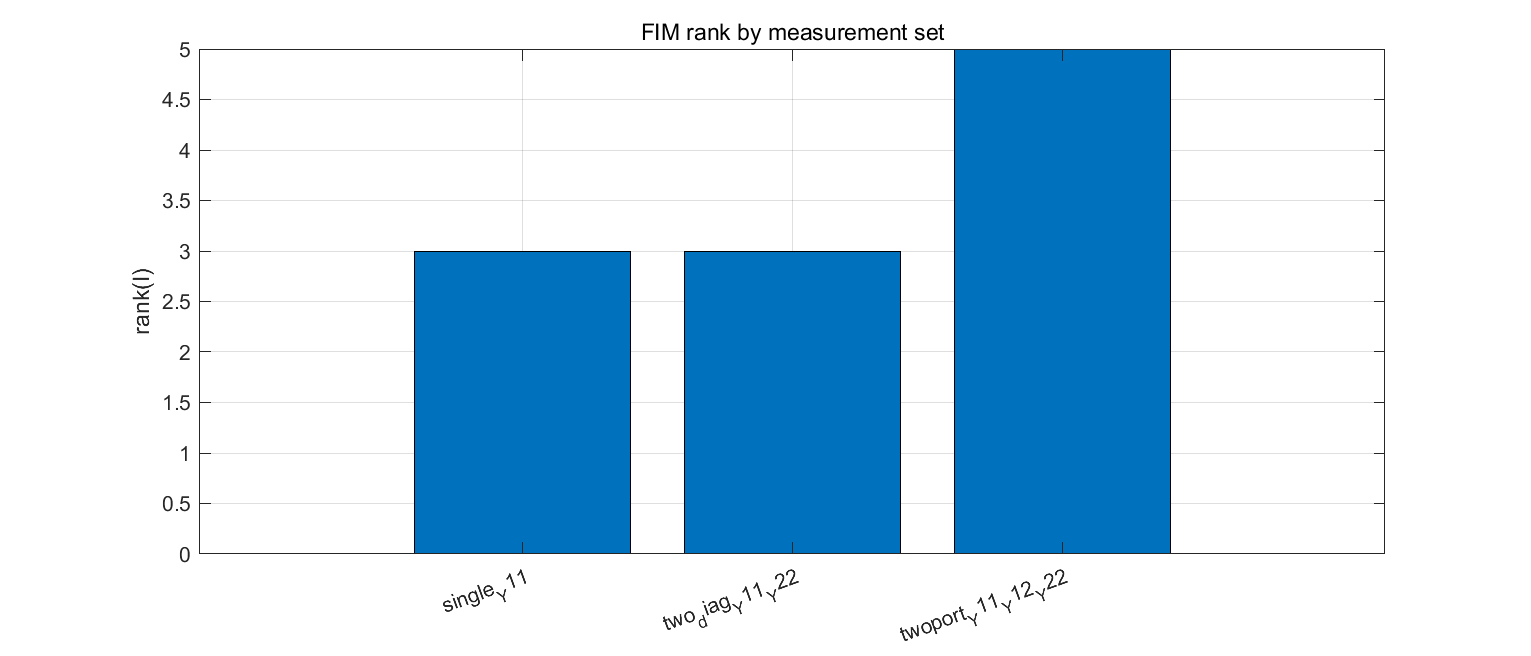
\includegraphics[width=\linewidth]{fim_rank.png}
\caption{不同观测集合的 Fisher 秩。}
\end{subfigure}\hfill
\begin{subfigure}[t]{0.47\textwidth}
\centering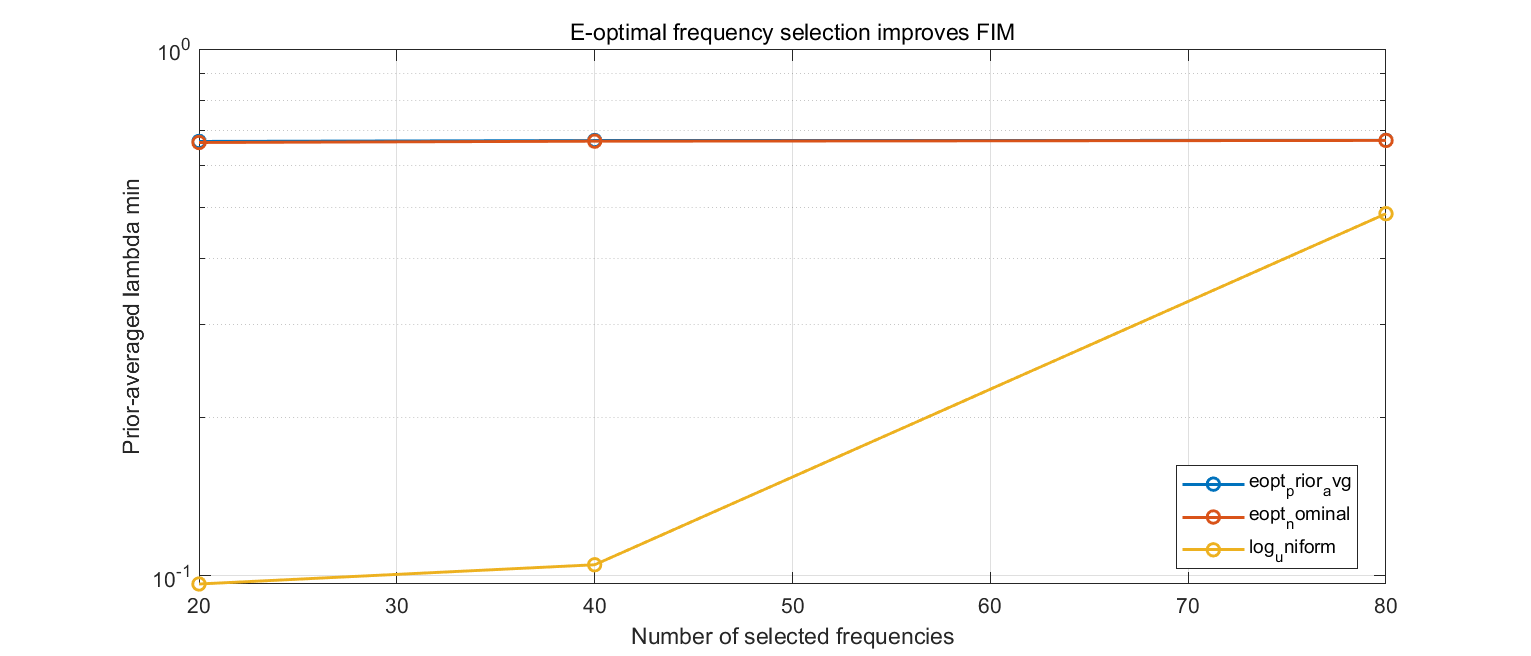
\includegraphics[width=\linewidth]{oed_lambda.png}
\caption{E-optimal 选频对最小信息特征值的改善。}
\end{subfigure}
\caption{Fisher/OED 给出“能否辨识、需要哪些端口与频点”的边界。GNN 只能在这个边界内利用结构先验降低方差，不能使不可观测方向凭空可见。}
\label{fig:fisher}
\end{figure}

\subsection{从整体参数走向分布参数：EXP-010 暴露了真正难点}

EXP-010 将整体两端口模型扩展为 $4+4$ 分段双梯形网络，候选参数为四个局部 $C_{ps,i}$。矩阵雅可比在数值上满秩，但第 2--4 段灵敏度相关系数高达 $0.992$--$0.996$，Fisher 条件数约 $1.24\times10^3$。在 4800 次局部线性反演中：
\begin{itemize}
\item 精确四单元定位准确率为 $87.44\%$；
\item 端部/内部区域定位准确率为 $93.73\%$；
\item 单元幅值平均绝对误差约 $30.51\%$；
\item 区域幅值平均绝对误差约 $41.60\%$。
\end{itemize}

这个结果的含义不是“算法已经很好”，而是：\textbf{端口频响对局部位置的分辨率有限；满秩不等于稳定可辨识；越细的参数化越容易产生高度相似的灵敏度列。} 这正是 GNN 方向的出发点，但 GNN 的目标应是学习合理的结构先验与区域化表示，而不是声称消除信息缺失。

\subsection{分段实验：端口等效不保证内部状态等效}

EXP-012 使用 $24+24$ 精细模型比较均匀、按层和信息引导连续分段。所有方法都可以获得很小的端口误差，但粗分段的最大相邻区段电压应力误差可超过 $9\%$；信息引导方法在每侧 8 段时满足当时设定的全部阈值，在每侧 12 段时内部峰值误差约 $0.0019\%$、相邻电压应力误差约 $0.441\%$，矩阵维度由 48 降为 24。

\begin{figure}[H]
\centering
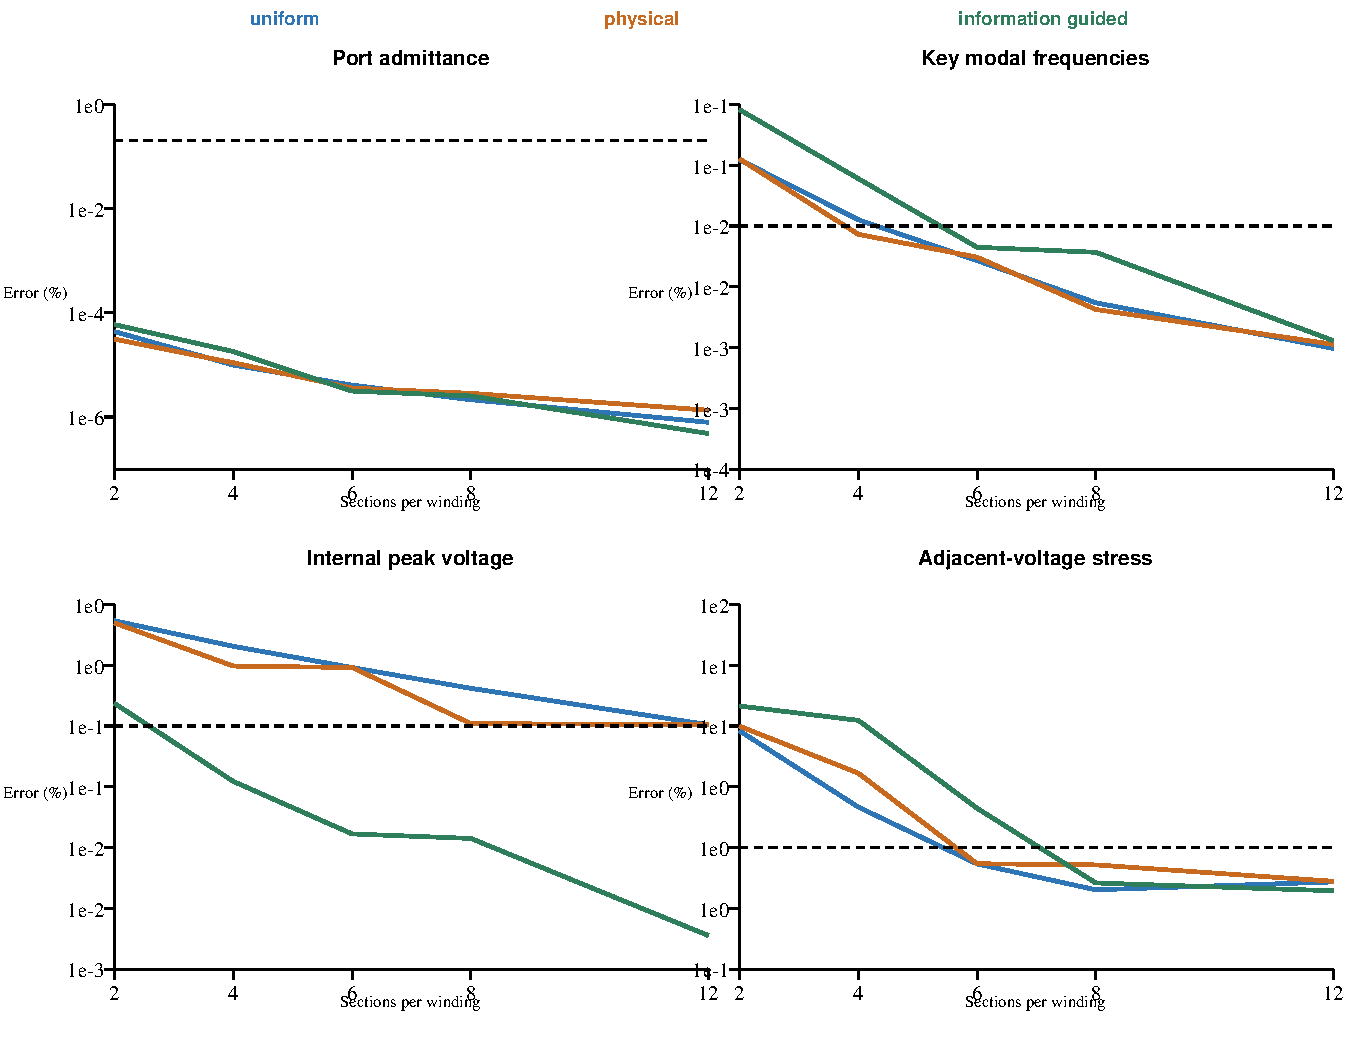
\includegraphics[page=1,width=0.96\textwidth]{segmentation_comparison.pdf}
\caption{EXP-012 分段策略比较。当前“信息引导”评分仍使用了精细模型内部电压这一 oracle 信息，因此它是方法探索，不是终端观测可直接实现的最终算法。}
\label{fig:segmentation}
\end{figure}

这一实验给 GNN 两个约束：其一，损失函数不能只有端口 $\Yp$；其二，若真实系统没有内部测量，训练时可用精细模型内部状态作监督，但部署时必须仅依赖端口观测和已知结构。

\section{梯形到广义全耦合图：统一矩阵方程}

\subsection{图对象与电路对象的一一对应}

定义异构图 $\mathcal G=(\mathcal V,\mathcal E)$：
\begin{itemize}
\item \textbf{PotentialNode}：绕组抽头、端子、内部电位节点与参考地；
\item \textbf{ConductorSegment}：具有 $R_i,L_{ii}$ 的导体区段；
\item \textbf{MagneticEdge}：任意两区段间互感 $M_{ij}$；
\item \textbf{CapacitanceEdge}：纵向、对地、跨绕组及屏蔽相关电容；
\item \textbf{ConductanceEdge}：介质损耗或泄漏支路；
\item \textbf{GeometricEdge}：只提供相对位置、距离、重叠、材料界面等几何先验，不直接进入 KCL。
\end{itemize}

若只保留相邻串联支路、相邻纵向电容及一一对应的跨绕组电容，就退化为经典双梯形；允许 $M_{ij}$ 和 $C_{ps,ij}$ 非局部连接、一次二次段数不同、屏蔽/磁芯/地作为额外节点时，就得到本文所称的广义“星形/全耦合图”。

\begin{figure}[H]
\centering
\begin{tikzpicture}[>=Latex,node distance=0.92cm and 1.35cm,
pn/.style={circle,draw=blue,fill=lightblue,minimum size=6mm,font=\small},
sn/.style={circle,draw=orange,fill=orange!12,minimum size=6mm,font=\small},
lab/.style={font=\small,align=center}]
\foreach \x in {0,...,5}{\node[pn] (p\x) at (1.45*\x,2.2) {$p_{\x}$};}
\foreach \x in {0,...,7}{\node[sn] (s\x) at (1.05*\x,0) {$s_{\x}$};}
\foreach \x [evaluate=\x as \y using int(\x+1)] in {0,...,4}{\draw[thick,blue] (p\x)--node[above,lab] {$R,L$}(p\y);}
\foreach \x [evaluate=\x as \y using int(\x+1)] in {0,...,6}{\draw[thick,orange] (s\x)--(s\y);}
\draw[dashed,green!70!black] (p0) to[bend right=12] node[left,lab] {$C_{ps,00}$}(s0);
\draw[dashed,green!70!black] (p1) to[bend right=12] (s2);
\draw[dashed,green!70!black] (p2) to[bend right=8] (s3);
\draw[dashed,green!70!black] (p2) to[bend left=20] (s6);
\draw[dashed,green!70!black] (p4) to[bend left=12] (s5);
\draw[dashed,green!70!black] (p5) to[bend left=12] (s7);
\draw[red!70!black,dotted,thick] (p0) to[bend left=28] node[above,lab] {$M_{05}$}(p5);
\draw[red!70!black,dotted,thick] (p1) to[bend left=22] (s6);
\node[lab,blue] at (3.65,3.05) {一次侧 $N_p=5$ 段};
\node[lab,orange!80!black] at (3.65,-0.8) {二次侧 $N_s=7$ 段};
\node[lab,green!50!black] at (9.2,1.4) {虚线：稀疏/非局部电容\\点线：全局磁耦合};
\end{tikzpicture}
\caption{从规则双梯形到非等段、非局部、全耦合图的概念演变。}
\label{fig:graphconcept}
\end{figure}

\subsection{支路矩阵与节点导纳矩阵}

设共有 $n_b$ 条导体支路、$n_v$ 个非参考电位节点。支路--节点关联矩阵 $\Inc\in\mathbb R^{n_v\times n_b}$ 的每一列在支路起点取 $+1$、终点取 $-1$。导体支路阻抗矩阵为
\begin{equation}
\bm Z_b(s)=\RR+s\LL,
\end{equation}
其中 $\RR=\operatorname{diag}(R_1,\ldots,R_{n_b})$，$\LL$ 的对角元为自感、非对角元为互感。支路电压、电流满足
\begin{equation}
\bm u_b=\Inc^T\vv,\qquad
\bm i_b=\bm Z_b^{-1}\bm u_b.
\end{equation}
把导体支路电流组装回节点，并加入节点电容矩阵 $\CC$ 与电导矩阵 $\GG$，得到统一节点方程
\begin{equation}
\boxed{
\bm Y_n(s)\vv=ii_{\mathrm{ext}},\qquad
\bm Y_n(s)=\Inc(\RR+s\LL)^{-1}\Inc^T+\GG+s\CC.}
\label{eq:nodal}
\end{equation}

任意一条节点 $a$ 与 $b$ 之间的电容 $c_e$，通过向量 $\bm d_e=\bm e_a-\bm e_b$ 装配：
\begin{equation}
\CC\leftarrow\CC+c_e\bm d_e\bm d_e^T.
\end{equation}
因此只要 $c_e\ge0$，单条电容边天然贡献半正定矩阵；互感矩阵通过 Cholesky 或物理耦合系数参数化保证 $\LL\succ0$。这为 GNN 输出提供了可实现的物理参数化，而不是训练后再修补无源性。

\subsection{端口 Kron 消元与内部状态}

把节点按端口 $p$ 和内部节点 $i$ 排列：
\begin{equation}
\begin{bmatrix}\ii_p\\\bm 0\end{bmatrix}
=
\begin{bmatrix}
\bm Y_{pp}&\bm Y_{pi}\\
\bm Y_{ip}&\bm Y_{ii}
\end{bmatrix}
\begin{bmatrix}\vv_p\\\vv_i\end{bmatrix}.
\end{equation}
内部节点无外加电流时，
\begin{equation}
\vv_i=-\bm Y_{ii}^{-1}\bm Y_{ip}\vv_p,
\end{equation}
端口导纳为
\begin{equation}
\boxed{
\Yp=\bm Y_{pp}-\bm Y_{pi}\bm Y_{ii}^{-1}\bm Y_{ip}.}
\label{eq:kron}
\end{equation}
式~\eqref{eq:nodal}--\eqref{eq:kron} 同时输出端口频响、内部节点电压、导体支路电流以及每条跨绕组电容的位移电流：
\begin{equation}
i_{ps,ab}(s)=sC_{ps,ab}\,[v_a(s)-v_b(s)].
\end{equation}
这就是 GNN 训练所需的“可微物理层”。

\section{Simscape 四端口模型与矩阵模型如何结合}

EXP-011 验证了矩阵模型与 Simscape 线性化模型的端口导纳一致性。其作用不是让 Simulink 代替矩阵求解，而是形成两种互补证据：矩阵模型便于扫频、求导和大规模训练；Simscape 便于检查电气连接、初始条件、求解器设置与开关时域行为。

\begin{figure}[H]
\centering
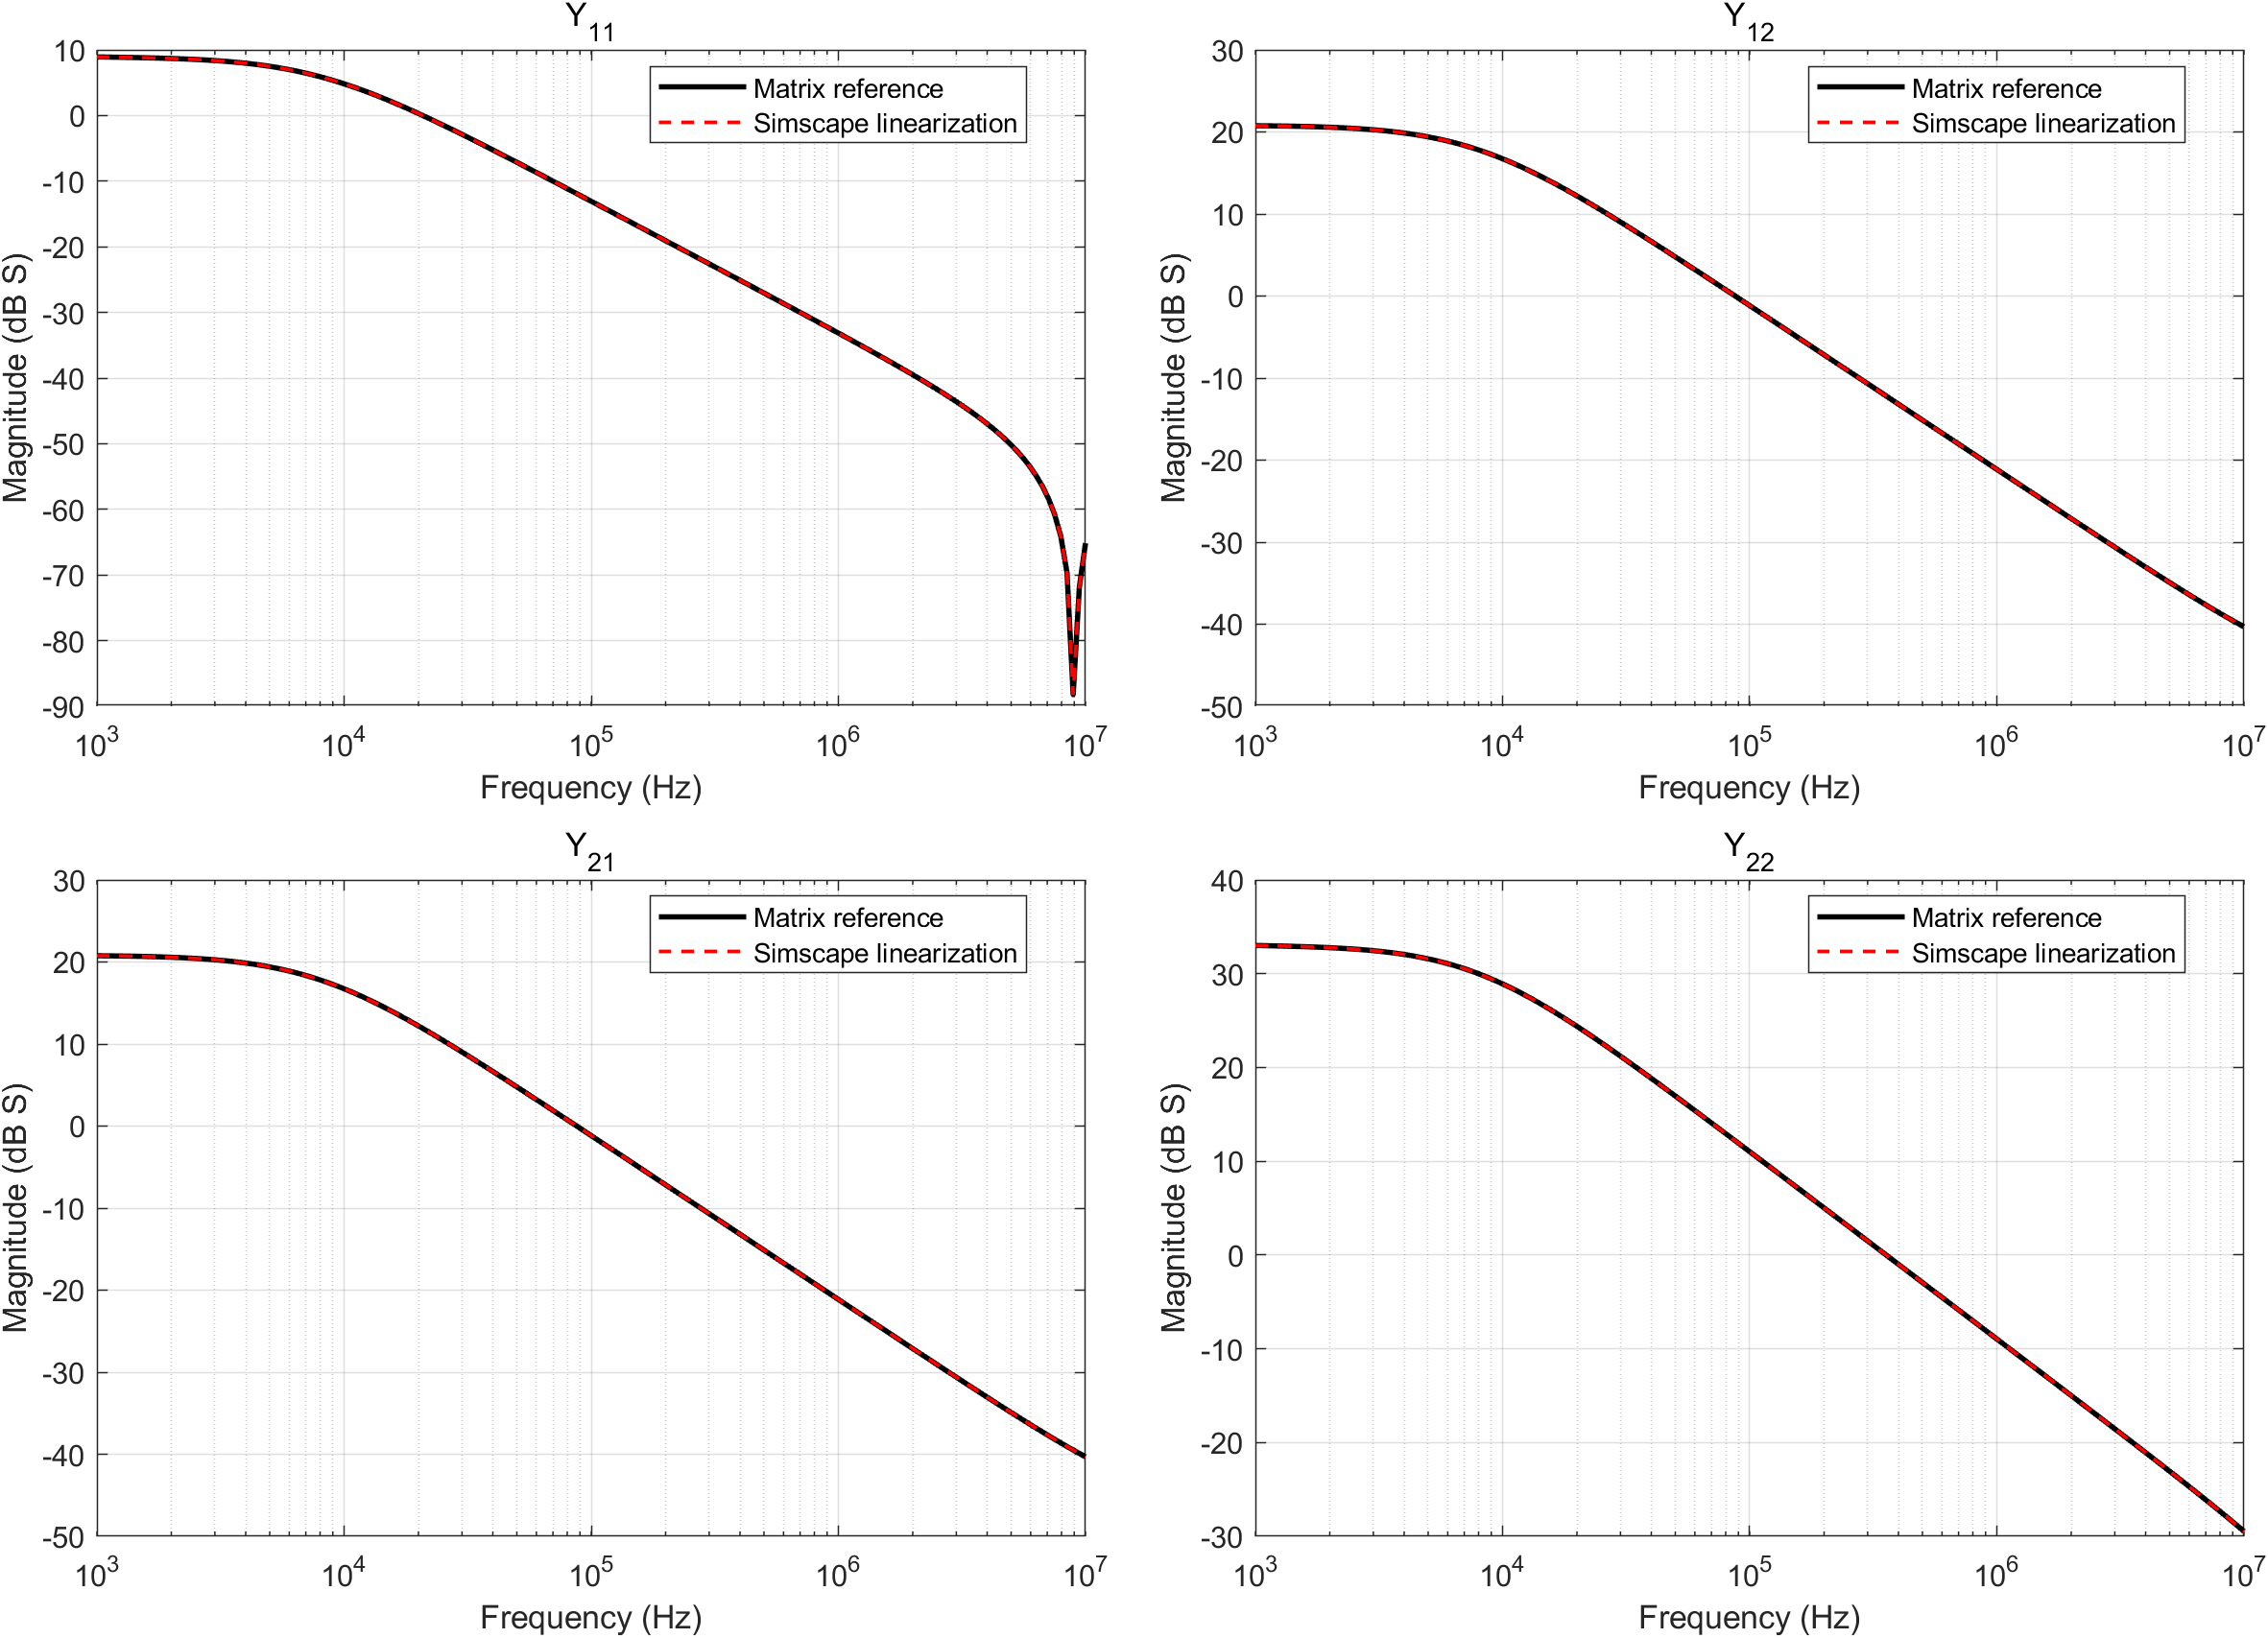
\includegraphics[width=0.92\textwidth]{simscape_matrix_validation.png}
\caption{Simscape 线性化与矩阵参考解的四个两端口导纳元素对比。曲线重合证明装配方程与物理电路实现的一致性。}
\label{fig:simscape-validation}
\end{figure}

\begin{figure}[H]
\centering
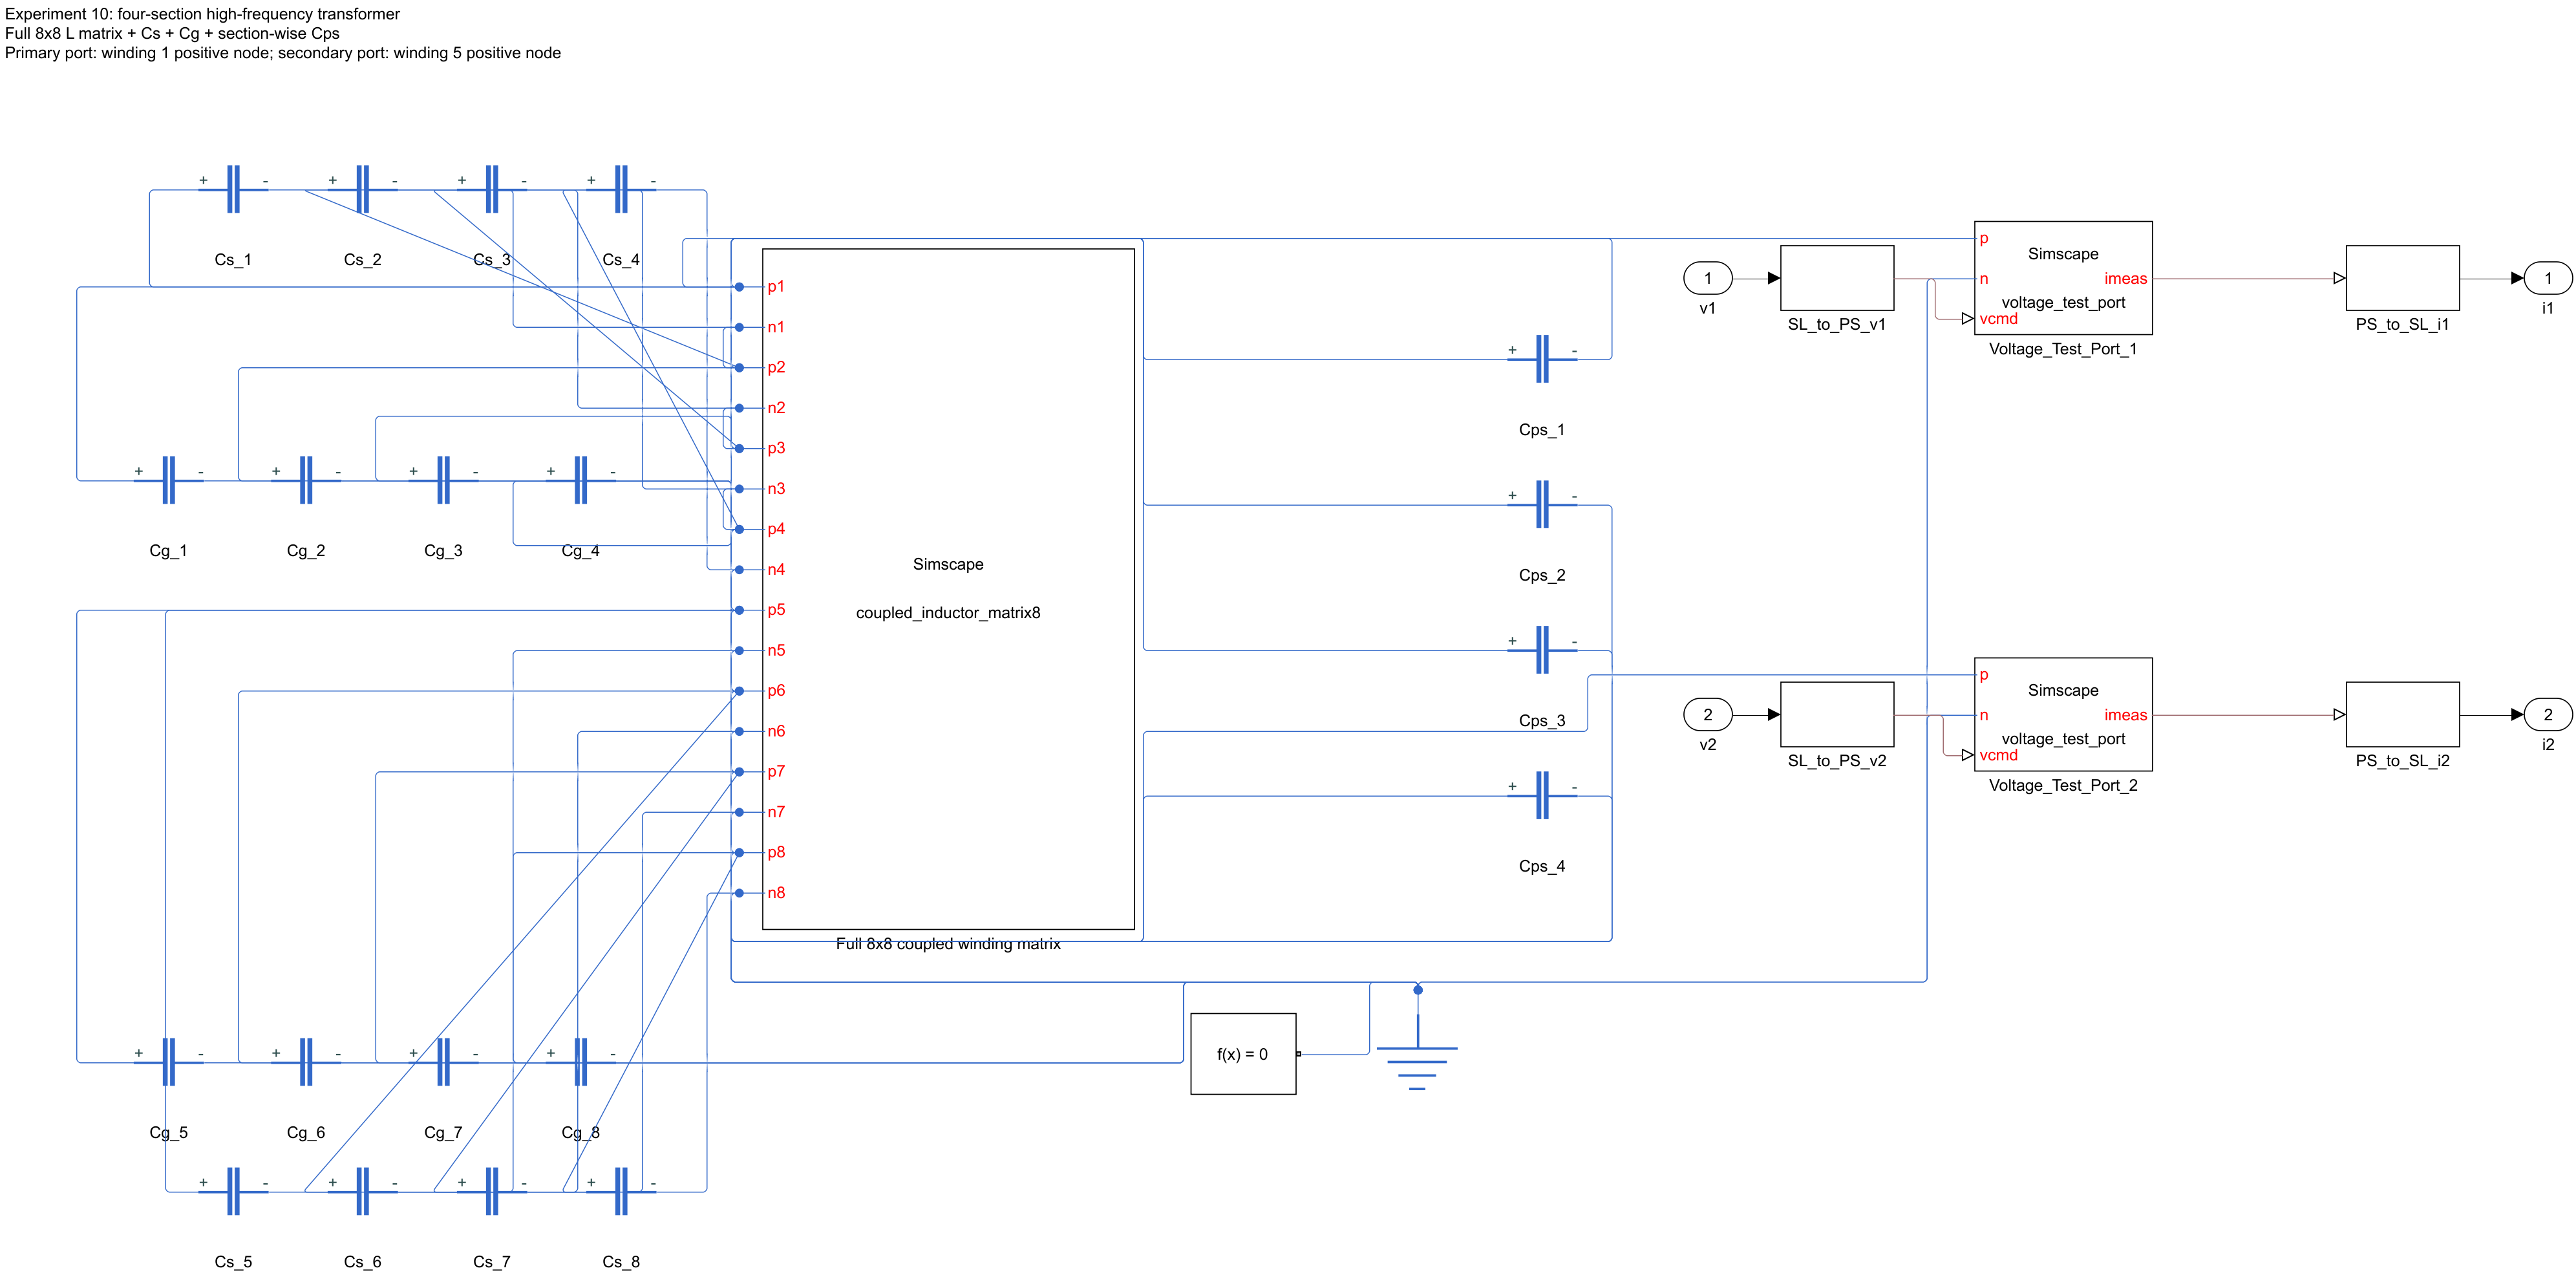
\includegraphics[width=0.84\textwidth]{simscape_model_overview.png}
\caption{程序化生成的分段高频变压器 Simscape 模型总览。该模型是仓库代码按 $R,L,C,M$ 网络自动搭建的，不是 Simulink 内置的“现成高频变压器内部结构”。}
\label{fig:simscape-overview}
\end{figure}

EXP-013 进一步构造一次、二次四个独立端子的参数化模型，允许 $N_p\ne N_s$、任意对称正定 $\LL$ 以及稀疏非局部 $\bm C_{ps}\)。这一步把“端口等效器件”升级成可以观测内部电压与局部位移电流的结构模型。

\begin{figure}[H]
\centering

\includegraphics[height=0.62\textheight,keepaspectratio]{four_terminal_8x8.png}
\caption{$8+8$ 四端口参数化高频变压器候选模型。图较密集恰好说明手工搭建不再可扩展，图--矩阵--Simscape 自动生成链路是必要的。}
\label{fig:fourterminal}
\end{figure}

EXP-014 把该 HFT 子系统接入双有源桥开关工况，采用 SPS $20\,\mathrm{kHz}$、相移 $30^\circ$、$400/100\,\mathrm{V}$，并用 $1\,\mu\mathrm{s}$ 有限边沿和 $100\,\mathrm{ns}$ Backward Euler 步长完成回归测试。当前功率不平衡用于暴露合成模型尚未稳态，并不作为效率结论。

\begin{figure}[H]
\centering
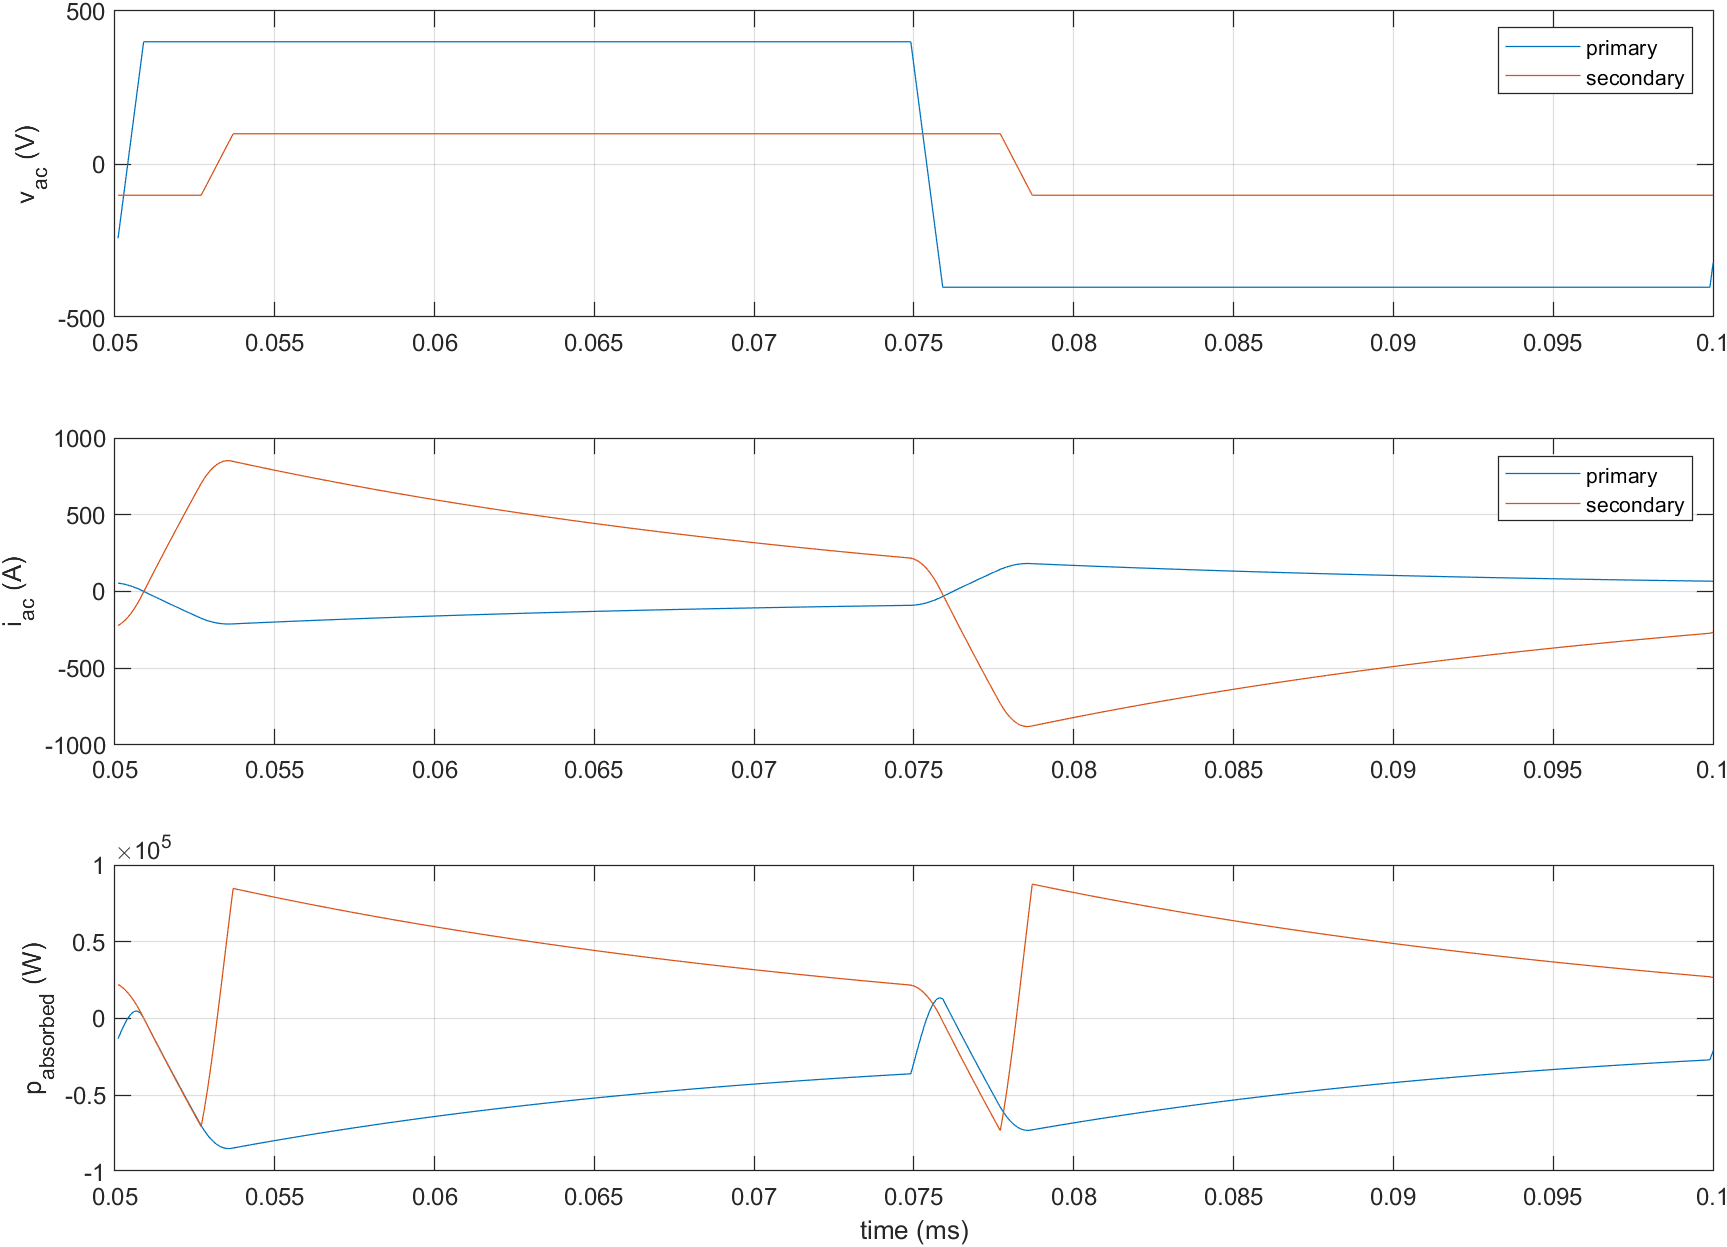
\includegraphics[width=0.91\textwidth]{dab_waveforms.png}
\caption{EXP-014 DAB 开关级回归波形。其价值是验证四端口模型可以进入实际拓扑并产生端口和内部观测，而不是证明当前合成参数代表某台真实样机。}
\label{fig:dab}
\end{figure}

最终的结合方式为：
\begin{enumerate}
\item 图数据结构保存拓扑、参数、几何和端口定义；
\item 确定性装配器生成 $\Inc,\RR,\LL,\CC,\GG$；
\item PyTorch 复数求解器执行式~\eqref{eq:nodal}--\eqref{eq:kron}，用于训练与梯度；
\item 同一图模型导出 Simscape 子系统，用于开关时域与工程连接验证；
\item 实测或 Simscape 产生端口观测，反演结果再回写图参数，闭环比较 $\Yp$、内部电压及局部位移电流。
\end{enumerate}

\section{已有 GitHub 工程给我们的具体启发}

EXP-015 对三个开源方向进行了固定提交版本的本地审计。结论不是直接复用某个仓库，而是吸收其表示与训练思想。

\begin{table}[H]
\centering
\small
\begin{tabularx}{\textwidth}{>{\bfseries}p{2.1cm}p{3.15cm}X X}
\toprule
工程 & 本地审计提交 & 可借鉴之处 & 不应照搬之处\\
\midrule
FALCON & \texttt{845145c0} & 电路关系类型、网表到图、图上反向优化的组织方式 & 目标电路域与 HFT 的互感/电容矩阵约束不同；当前环境缺 PyG，未完成原仓库端到端运行\\
GraphGPS & \texttt{28015707} & 局部消息传递与全局注意力并联，适合同时建模邻接梯形边与远距离耦合 & GraphGym 配置体系较重；不能把所有边当同一种关系\\
EGNN & \texttt{e9ca6c0c} & 相对几何编码、平移旋转等变思想；本地小型前后向已通过 & HFT 绕组坐标是已知物理结构，不应在消息传递中任意更新坐标\\
\bottomrule
\end{tabularx}
\caption{GitHub 工程认知及其对本项目的边界。提交号用于保证审计可复现，不代表这些仓库的最新状态。}
\label{tab:github}
\end{table}

据此，推荐骨干不是“纯 GCN”或“纯 Transformer”，而是：
\begin{equation}
\boxed{\text{typed local MPNN}+\text{GPS global attention}+\text{fixed-coordinate relative geometry}.}
\end{equation}
局部 MPNN 处理串联、纵向电容、对地等明确关系；全局注意力处理稠密互感与非局部跨绕组耦合；几何编码只作为特征，不改变真实坐标。

\section{物理图求解器已经完成了什么}

EXP-015 已实现从异构图到矩阵的确定性装配，以及 PyTorch 复数可微求解器。$4+4$ 与 $8+8$ 图模型相对旧矩阵求解器的端口误差分别为 $2.06\times10^{-15}$ 与 $4.95\times10^{-15}$；最大内部 KCL 残差约 $2.0\times10^{-14}\,\mathrm{A}$；$R$、自感、互感、对地电容和跨绕组电容均完成自动微分/有限差分检查。运行环境检测到 PyTorch 2.11.0+cu128 与 CUDA。

这意味着 GNN 的前置条件已经具备：
\begin{equation}
\mathcal G(\bm\theta)
\xrightarrow{\text{assembly}}
(\Inc,\RR,\LL,\CC,\GG)
\xrightarrow{\text{complex solve}}
(\Yp,\vv_i,\bm i_b,\bm i_{ps}),
\end{equation}
且右端对 $\bm\theta$ 可导。后续无需让网络“记住电路响应”，网络输出的参数可以直接送入真实方程验算。

\section{GNN 应解决的逆问题}

\subsection{为什么简单最小二乘不够}

整体 $\Cps$ 与 $\Ls$ 的低维联合最小二乘是必要基线，但分布模型的未知量很快增长：
\begin{equation}
\bm\theta=
[R_i,L_{ii},M_{ij},C_{s,i},C_{g,i},C_{ps,ij},G_{ij}]^T.
\end{equation}
若有 $N_p+N_s=N$ 个区段，完整互感项可达 $O(N^2)$，跨绕组电容可达 $O(N_pN_s)$。端口观测维度却没有同比增长，导致强相关、病态与多解。经典最小二乘只利用当前样本的数值残差，不知道“相邻区段往往共同变化”“异常通常稀疏”“同一种结构在不同尺寸上具有共享规律”。

\subsection{推荐任务：基线已知下的结构化增量辨识}

第一版不应让 GNN 从零恢复全部绝对参数，而应假设健康基线 $\bm\theta_0$ 由设计、离线扫频或 FEM 标定，在线识别相对变化：
\begin{equation}
\bm\theta=\bm\theta_0\odot\exp(\Delta\bm z).
\end{equation}
对电容、电阻和自感使用对数增量保证正值；互感可用有界耦合系数或 Cholesky 因子参数化，从构造上保持 $\LL\succ0$。输出分成三层：
\begin{enumerate}
\item 全局头：$\Delta C_{ps}^{\mathrm{total}},\Delta L_{\sigma}^{\mathrm{eq}}$，与已有整体辨识对齐；
\item 区域头：端部/中部/屏蔽附近等可辨识区域的异常概率和幅值；
\item 边级头：只有在 Fisher 分辨率允许时才输出 $\Delta C_{ps,ij},\Delta M_{ij}$ 等局部参数及不确定度。
\end{enumerate}

\subsection{网络输入与双编码器结构}

每个图节点/边的静态特征包括类型、绕组侧别、归一化轴向/径向位置、长度、截面积、材料、距离、重叠面积和健康参数。动态观测不是简单拼到每个节点，而由频谱编码器处理：
\begin{equation}
\bm x_k=
[\operatorname{PE}(\log f_k),\operatorname{Re}\bm Y_{\mathrm p,k},
\operatorname{Im}\bm Y_{\mathrm p,k},q_k,\gamma_k^2,\bm u_k],
\end{equation}
其中 $q_k$ 为 Fisher/OED 信息得分，$\gamma_k^2$ 为相干度，$\bm u_k$ 为运行窗口条件。由此形成：
\begin{equation}
\begin{aligned}
\bm H_G &= \operatorname{GraphEncoder}(\mathcal G_0),\\
\bm H_F &= \operatorname{SpectralEncoder}(\{\bm x_k\}),\\
\Delta\widehat{\bm z} &=
\operatorname{EdgeDecoder}\!\left(
\operatorname{CrossAttention}(\bm H_G,\bm H_F)\right).
\end{aligned}
\end{equation}
图编码器负责“结构上谁与谁相关”，频谱编码器负责“观测中哪些频率/端口出现了什么证据”，交叉注意力负责把端口证据分配给候选节点和边。

\begin{figure}[H]
\centering
\begin{tikzpicture}[scale=0.78,transform shape,node distance=0.8cm and 0.95cm,>=Latex,
box/.style={rounded corners,draw=navy,fill=lightblue,minimum height=1.05cm,text width=2.8cm,align=center,font=\small},
phys/.style={rounded corners,draw=green!60!black,fill=green!10,minimum height=1.05cm,text width=3.0cm,align=center,font=\small},
loss/.style={rounded corners,draw=orange!80!black,fill=orange!12,minimum height=0.9cm,text width=2.7cm,align=center,font=\small}]
\node[box] (g) {健康基线异构图\\几何、类型、$\bm\theta_0$};
\node[box,right=of g] (ge) {Typed MPNN\\+ GPS 全局注意力};
\node[box,below=of g] (y) {OED 多端口频谱\\$\Yp(f),q_f,\gamma^2$};
\node[box,right=of y] (se) {轻量频谱编码器\\复数令牌与工况};
\node[box,right=1.15cm of ge,yshift=-0.9cm] (cross) {图--频谱\\交叉注意力};
\node[box,right=of cross] (dec) {层级解码器\\全局/区域/边级};
\node[phys,right=of dec] (solver) {物理可微层\\图$\to A,R,L,C,G$\\Kron/内部状态};
\node[loss,below=of solver] (l) {复频响、内部状态、\\稀疏性与物理约束损失};
\draw[->,thick] (g)--(ge); \draw[->,thick] (y)--(se);
\draw[->,thick] (ge)--(cross); \draw[->,thick] (se)--(cross);
\draw[->,thick] (cross)--(dec); \draw[->,thick] (dec)--node[above,font=\scriptsize] {$\Delta\hat{\bm z},\hat\sigma$}(solver);
\draw[->,thick] (solver)--(l); \draw[->,thick,bend right=18] (l.west) to (dec.south);
\end{tikzpicture}
\caption{建议的物理约束图反演架构。主干是 GNN，频谱模块负责观测编码，最终预测必须经过同一个矩阵求解器验算。}
\label{fig:architecture}
\end{figure}

\subsection{目标函数：数据、结构与物理三类约束}

推荐的总损失为
\begin{equation}
\mathcal L=
\lambda_Y\mathcal L_Y+
\lambda_\theta\mathcal L_{\theta}+
\lambda_{int}\mathcal L_{int}+
\lambda_{sp}\mathcal L_{sp}+
\lambda_{tv}\mathcal L_{tv}+
\lambda_{phy}\mathcal L_{phy}+
\lambda_u\mathcal L_u.
\end{equation}
其中：
\begin{align}
\mathcal L_Y&=\sum_{k\in\mathcal K}
\left\|\bm\Sigma_k^{-1/2}
[\bm Y_{\mathrm p}(f_k;\widehat{\bm\theta})-\widehat{\bm Y}_{\mathrm p,k}]\right\|_F^2,\\
\mathcal L_{\theta}&=\|\Delta\widehat{\bm z}-\Delta\bm z^{\star}\|_1,\\
\mathcal L_{int}&=\sum_k\|\widehat{\vv}_i(f_k)-\vv_i^{\star}(f_k)\|_2^2,\\
\mathcal L_{sp}&=\sum_{g\in\mathcal G_{grp}}\|\Delta\widehat{\bm z}_g\|_2,\\
\mathcal L_{tv}&=\sum_{(e,e')\in\mathcal N_E}w_{ee'}
|\Delta\hat z_e-\Delta\hat z_{e'}|,\\
\mathcal L_{phy}&=\mathcal P(\widehat{\LL}\not\succ0)+
\|\widehat{\Yp}-\widehat{\Yp}^{,T}\|_F^2+
\mathcal P(\operatorname{Re}\widehat{\Yp}\not\succeq0).
\end{align}
$\mathcal L_u$ 可采用异方差负对数似然，使模型在低相干度、低 Fisher 信息或分布外工况下给出更大的不确定度。没有分布参数真值时，$\mathcal L_{\theta}$ 与 $\mathcal L_{int}$ 可以在训练仿真中使用；真实部署主要依靠 $\mathcal L_Y$、全局守恒、物理约束和少量校准标签。

\section{已有 AI 残差试验应怎样定位}

早期 AI 试验使用轻量网络修正整体 $\Cps$ 物理估计，插值结果显示修正点更贴近真值。这证明“物理锚点 + 数据残差”可行，但它仍是低维标量问题，无法体现拓扑、变规模与局部耦合。

\begin{figure}[H]
\centering
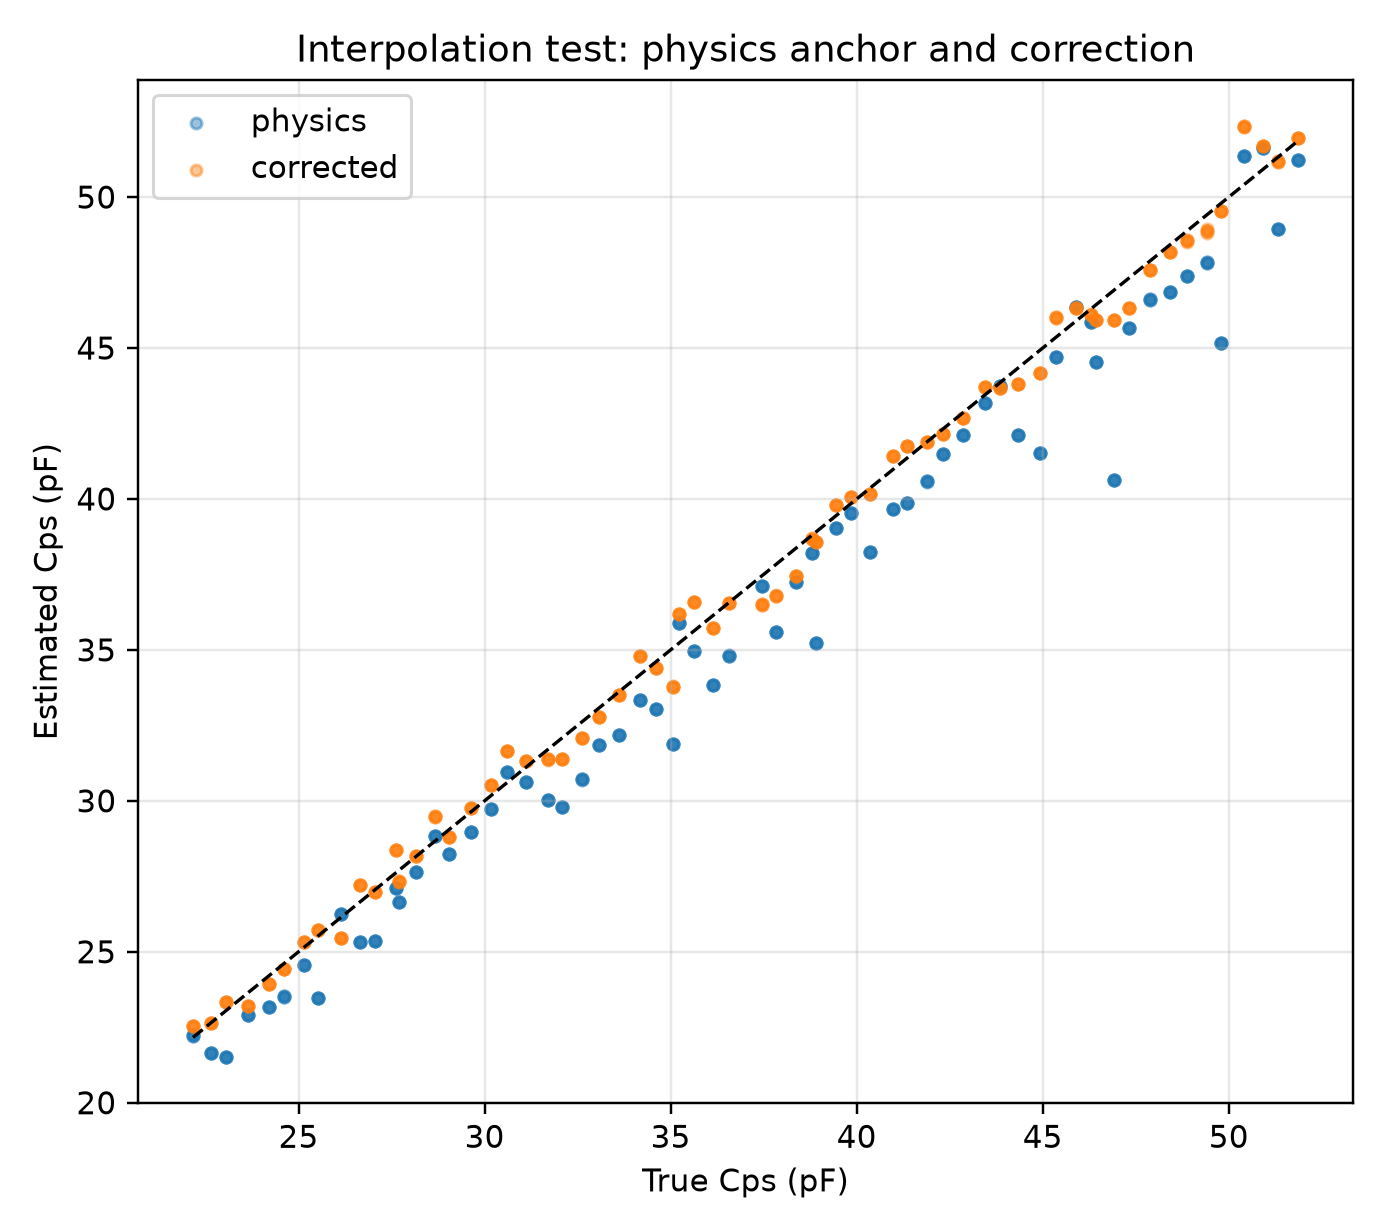
\includegraphics[width=0.68\textwidth]{ai_residual_pilot.png}
\caption{已有整体 $\Cps$ 残差学习试验。它应作为 AI 可行性先导和对照组，而不是未来 GNN 论文的核心贡献。}
\label{fig:aipilot}
\end{figure}

GNN 方向相对它的实质升级是：
\begin{equation}
\text{标量残差}quad\longrightarrow\quad
\text{拓扑条件化的边级/区域级结构化逆问题}.
\end{equation}

\section{数据从哪里来，质量怎样把握}

\subsection{三层数据而不是一次生成海量样本}

\begin{enumerate}
\item \textbf{解析/矩阵层：}用可微图求解器快速生成大规模参数扰动数据，覆盖稀疏局部变化、连续区域变化和耦合边组合；适合预训练。
\item \textbf{Simscape/DAB 层：}引入开关边沿、死区、$C_{oss}$、负载、接地和测量链路，制造 forward model 与 inverse model 的失配；适合困难样本微调。
\item \textbf{FEM/实测层：}数量少但权威，用于校准参数分布、验证非局部耦合和最终迁移；不需要一开始就拥有大规模实机故障数据。
\end{enumerate}

第一版可使用 $10^4$--$5\times10^4$ 个矩阵样本预训练，再选择约 $10^3$--$5\times10^3$ 个高信息 Simscape 样本微调；具体数量应由学习曲线决定，不应预先承诺。CUDA 主要加速 GNN、批量复数矩阵求解和自动微分，Simscape 数据生成仍主要受 CPU 与求解器影响。

\subsection{数据正确性的五道检查}

\begin{enumerate}
\item \textbf{矩阵物理性：}$\RR\succeq0,\LL\succ0,\CC\succeq0,\GG\succeq0$；
\item \textbf{网络守恒：}内部 KCL 残差、端口互易误差、正实性；
\item \textbf{双实现一致：}随机抽样用 Simscape 线性化对照矩阵 $\Yp$；
\item \textbf{逆问题难度标注：}保存 Fisher 特征值、灵敏度相关性和可辨识区域标签；
\item \textbf{防止数据泄漏：}按结构/工况/扰动区域分组划分，而不是随机拆分相邻参数点。
\end{enumerate}

\section{实验设计：怎样证明 GNN 确实解决了复杂辨识问题}

\subsection{基线与消融}

\begin{table}[H]
\centering
\small
\begin{tabularx}{\textwidth}{p{3.0cm}X X}
\toprule
方法 & 回答的问题 & 必须报告的边界\\
\midrule
非线性最小二乘 & 物理模型单独能做到什么 & 初值、正则、运行时间、局部极小值\\
Group Lasso/TV & 稀疏与连续先验是否已经足够 & 正则系数敏感性\\
MLP/1D-CNN & 不使用图拓扑的数据驱动基线 & 固定维度与跨结构能力\\
Typed MPNN & 局部关系类型是否有效 & 远程耦合能力\\
MPNN+GPS & 全局互感/跨绕组耦合是否需要注意力 & 参数量、计算复杂度\\
完整 Physics-GNN & 物理层、Fisher、层级头是否共同有效 & 去掉每个模块的消融\\
\bottomrule
\end{tabularx}
\caption{推荐的对照方法。简单方法必须保留；高级网络的价值要通过困难划分和消融证明。}
\end{table}

\subsection{评价指标必须覆盖端口、参数和内部工程量}

建议同时报告：
\begin{itemize}
\item 全局总量误差：$\Cps^{total},\Ls^{eq}$；
\item 区域/边定位：Top-1、Top-$k$、端部/内部区域准确率、AUPRC；
\item 幅值：对数 MAE、相对误差、校准后的置信区间覆盖率；
\item 端口：$Y_{pq}$ 逐元素幅相误差、谐振/反谐振位置；
\item 内部：最大节点电压、最大相邻区段电压及位置、局部 $i_{ps}$；
\item 物理：KCL、互易性、无源性与 $\LL/\CC$ 正定性；
\item 工程：单次在线推理时间、所需窗口数、噪声/温度/接地/负载鲁棒性。
\end{itemize}

\subsection{最关键的测试划分}

随机划分只能证明插值。真正有价值的测试是：
\begin{enumerate}
\item 未见过的扰动位置；
\item 未见过的局部参数组合；
\item 未见过的 DAB 相移、负载与边沿时间；
\item $4+4$ 训练、$8+8$ 或 $N_p\ne N_s$ 测试；
\item 合成矩阵训练、Simscape 测试；
\item 仿真预训练、少量实测微调后的样机外测试。
\end{enumerate}

\section{下一步实施路线与停止条件}

\subsection{阶段 A：先固定逆问题，不立即追求大网络}

以 EXP-015 图物理求解器为底座，新增一套“健康图 + 稀疏/区域参数扰动 + 多端口频响”的数据生成器。第一批只辨识两类边：$C_{ps,ij}$ 与 $M_{ij}$（或局部 $L_i$），其余参数作为已知或小范围 nuisance。这样能直接复现 EXP-010 的强相关难题，又不会一次放开全部 $RLCG$。

停止条件：数据通过五道物理检查；最小二乘与 Group Lasso 基线已建立；Fisher 分析能够标出不可区分边组。

\subsection{阶段 B：建立最小可用 Physics-GNN}

先实现 typed MPNN + 层级边解码 + 可微物理损失，不加大型频谱 Transformer。观测频点使用已有 OED 方案。若局部 MPNN 在非局部耦合上明显受限，再加入一到两层 GPS 全局注意力。

停止条件：在相同观测下，相比 Group Lasso/TV 提升区域定位或幅值稳定性；端口拟合没有以违反无源性为代价；跨 $4+4\to8+8$ 测试优于固定维度 MLP。

\subsection{阶段 C：处理真实失配与迁移}

使用 EXP-014 DAB/Simscape 生成少量高成本样本，加入负载、温度代理参数、接地阻抗、探头增益/相位、死区与边沿变化。采用矩阵预训练、Simscape 微调；之后再接 FEM 或低压样机少样本适配。

停止条件：在 forward/inverse 不同模条件下优于纯物理反演；不确定度能在分布外工况增大；整体 $\Cps$ 与局部分布之和保持一致。

\subsection{阶段 D：再考虑自适应分段}

分段不是当前第一主线。只有当固定精细图的计算量成为瓶颈，或 Fisher 明确显示大量边只能成组辨识时，再引入学习式合并：将不可区分的相邻边聚为可辨识区域，并保证聚合后的 $\RR,\LL,\CC,\GG$ 仍满足物理约束。此时 AI 的作用是\textbf{选择可辨识模型分辨率}，而不是为了结构新颖而随意切段。

\section{风险、边界与最终判断}

\begin{enumerate}
\item \textbf{最大科学风险：}分布参数对端口观测本身不可区分。应通过 Fisher、灵敏度相关和区域合并诚实报告分辨率，不能用网络准确率掩盖先验主导。
\item \textbf{最大数据风险：}同模生成--同模反演得到近零误差。必须保留 Simscape/FEM/实测跨模型测试。
\item \textbf{最大工程风险：}合成参数并非真实样机参数。现阶段结论是算法链和物理实现成立，不是样机性能已被验证。
\item \textbf{最大 AI 风险：}网络过重而数据不足。应优先使用变规模图的结构优势和物理层，而不是追求参数量。
\end{enumerate}

\begin{keybox}
\textbf{最终判断：}这条 GNN 路线值得继续，而且比“给整体 $\Cps$ 最小二乘后点缀一个网络”更有技术壁垒。现有工作已经完成从整体可辨识性、分布病态性、矩阵/Simscape 一致性、四端口 DAB 接入到可微图求解器的前置闭环。下一步最有价值的不是再写一份概念网络，而是用现有物理求解器生成第一版结构化扰动数据，建立 Group Lasso 与 typed MPNN 两条可运行基线，并用 Fisher 结果决定边级还是区域级输出。
\end{keybox}

\clearpage
\section*{实验与代码来源索引}
\addcontentsline{toc}{section}{实验与代码来源索引}
\small
\setlength{\tabcolsep}{4pt}
\noindent
\begin{tabularx}{\textwidth}{p{1.8cm}X}
\toprule
编号 & 本报告使用的内容\\
\midrule
Legacy & Liu 三电容复现、PWM/多端口/Fisher/OED、整体 $\Cps$ 与位移电流闭环、AI 残差先导\\
EXP-010 & $4+4$ 分段梯形矩阵、局部 $C_{ps,i}$ 灵敏度与 4800 次反演\\
EXP-011 & 矩阵--Simscape 导纳一致性、程序化模型搭建\\
EXP-012 & $24+24$ 精细模型及均匀/按层/信息引导分段比较\\
EXP-013 & 任意 $N_p,N_s$ 的四独立端子全耦合参数化模型\\
EXP-014 & DAB SPS 开关级模型、有限边沿与时域回归\\
EXP-015 & 异构图 schema、图到矩阵装配、PyTorch 复数可微求解、GitHub 工程审计\\
\bottomrule
\end{tabularx}

\section*{参考资料}
\addcontentsline{toc}{section}{参考资料}
\begin{enumerate}
\item Liu 等：\emph{Experimental Extraction of Parasitic Capacitances for High-Frequency Transformers}, IEEE Transactions on Power Electronics, 2017.
\item 任富强：\emph{变压器绕组梯形等效网络参数辨识及其在连续式绕组变形诊断中的应用}，西安交通大学博士学位论文，2020.
\item FALCON repository，\url{https://github.com/mit-han-lab/FALCON}，本地审计提交 \texttt{845145c0}（完整哈希见仓库审计记录）。
\item GraphGPS repository，\url{https://github.com/rampasek/GraphGPS}，本地审计提交 \texttt{28015707}（完整哈希见仓库审计记录）。
\item EGNN repository，\url{https://github.com/lucidrains/egnn-pytorch}，本地审计提交 \texttt{e9ca6c0c}（完整哈希见仓库审计记录）。
\end{enumerate}

\end{document}
(\Inc,\RR,\LL,\CC,\GG)
